\documentclass[a4paper,10pt]{report}
\usepackage[utf8]{inputenc}
\usepackage{color}
\usepackage{colortbl}
\usepackage{graphicx}
% Title Page
%\title{}
%\author{}

\definecolor{Gray}{gray}{0.8}
\definecolor{lightGray}{gray}{0.925}

\newcolumntype{A}{>{\columncolor{Gray}}c}
\newcolumntype{B}{>{\columncolor{Gray}}l}

\begin{document}
%\maketitle
\begin{titlepage}

\begin{center}
\begin{tabular}{|A|}
\hline
\\
\\
\\
\bfseries \Huge \quad \quad \quad  Pflichtenheft   \quad \quad \quad
\\
\\
\Large zum Softwareprojekt\\
\Large (Prof. Steinbach)\\
\\
\\
\hline
\end{tabular}
\end{center}

\vspace{3,5mm}

\begin{center}
\begin{tabular}{|A|}
%Hier Projektnamen einfügen.
%Bei Bedarf die \quad entfernen, sie dienen nur der einheitlichen Breite der Tabellen
\hline
\\
\\
\bfseries \Large \quad \quad \quad Struktogrammeditor (42) \quad \quad \quad
\\
\\
\\
\\
\hline
\end{tabular}
\end{center}

\vspace{9mm}

\bfseries \large Angaben zu den am Projekt beteiligten Studenten:

%\begin{center}
\begin{tabular}{|c|l|l|l|l|}
%Hier Mitglieder der Projektgruppe eintragen. Vor jeden Namen ein \normalsize setzen; wird die Tabelle durch lange Namen zu groß \normalsize durch \small ersetzen
\hline
\rowcolor{Gray}\small &\small Name, Vorname &\small Mat.-Nr. & Studiengang &\small Email-Adresse \\
\hline
\rowcolor{lightGray}\small 1. &\small Jonas Toth &\small 57319 & BAI &\small Jonas.Toth@student.tu-freiberg.de\\
\hline
\rowcolor{Gray}\small 2. &\small Christian Sacher &\small 57406 & BAI &\small Christian.Sacher@student.tu-freiberg.de \\
\hline
\rowcolor{lightGray}\small 3. &\small Martin Plank&\small 57464 &BAI &\small plank-martin@web.de  \\
\hline

\end{tabular} 
%\end{center}

\vspace{10mm}

\begin{center}
\begin{tabular}{|BB|}
\hline
\bfseries \large Best\"{a}tigt durch Prof. Steinbach & \quad \quad \quad \quad \quad \quad \quad \quad \quad \\
\bfseries \large Datum, Unterschrift &
\\
\hline
\end{tabular}
\end{center}

\end{titlepage}
%\begin{abstract}
%\end{abstract}

\newpage
\renewcommand{\thesection}{\arabic{section}}

\tableofcontents
\newpage

\section{Zielbestimmung}
Ziel des Softwareprojektes ist es, ein Programm zur Erzeugung und Visualisierung von Struktogrammen zu erstellen. 
Mit dessen Hilfe sollen Programmieranf\"{a}nger ein Tool in der Hand haben um Algorithmen und Programme systematisch zu verstehen und entwickeln.

\subsection{Musskriterien}
\begin{itemize}

\item Zusammensetzung des Struktogrammes aus einzelnen unabhängigen Elementen(siehe Glossar)
\item Verwaltung des Struktogrammes
\item GUI zur benutzerfreundlichen Visualisierung des Struktogrammes
\item Anlegen von Variablen innerhalb eines Struktogrammes
\item Verfügbare Datentypen: Basisdatentypen (String, Float, Integer, Boolean), eindimensionale Arrays der Basisdatentypen
\item Speichern und Laden von Struktogrammen


\end{itemize}

\subsection{Wunschkriterien}
\begin{itemize}
\item Visualisierung des Programmablaufes
\item Export zu gängigen Bildformaten
\item Mehrdimensionale Arrays der Basisdatentypen
\item Übersicht über Struktogramm in Anlehnung eines Dateibaumes
\end{itemize}

\subsection{Abgrenzungskriterien}
\begin{itemize}
\item Es soll kein funktionierendes Programm aus dem Struktogramm generiert werden
\item nur prozedurales Programmierparadigma durch Struktogramm beschreiben
\item Beschränkung auf 4 Basisdatentypen (String, Integer, Float, Boolean) d.h. keine Strukturen oder selbstdefinierte Datentypen
\end{itemize}
\newpage
\section{Produkteinsatz}
\subsection{Anwendungsbereiche}
Das Programm dient Programmieranfängern bei der Visualisierung und Entwicklung einfacher Algorithmen. Es soll mehr das grundsätzliche Verständnis von Programmen
veranschaulicht werden anstatt komplexe Programme entwickeln zu können. Das Programm kann zur Lehre in Modulen wie Prozedurale Programmierung eingesetzt werden.
\subsection{Zielgruppen}
\begin{itemize}
\item Schüler und Studenten
\item Informatikinteressierte Einsteiger
\end{itemize}
\subsection{Betriebsbedingungen}
\begin{itemize}
\item Das Programm soll auch von Anfängern benutzt werden können
\item Das Programm muss nicht beobachtet werden da es nur auf Input reagiert
\item Das Programm soll ohne Laufzeitbegrenzung sein
\end{itemize}
\section{Produktumgebung}
\subsection{Software}
\begin{itemize}
\item Windows 7 und Windows 10
\item C++/CLI in Kombination mit .NET 4.5
\end{itemize}
\subsection{Hardware}
\begin{itemize}
\item normaler Desktop PC (Maus, Tastatur, Monitor)
\end{itemize}
\subsection{Orgware}
\begin{itemize}
\item nicht nötig
\end{itemize}
\subsection{Produktschnittstellen}
\begin{itemize}
\item nicht nötig
\end{itemize}
\newpage
\section{Produktfunktionen}
\begin{itemize}
\item /F10/ Struktogramm aus einzelnen Elementen(siehe Glossar) zusammen setzen
\item /F20/ Auswahl der Art eines Elements via Dropdown Menü
\item /F30/ bestehenden Element löschen
\item /F40/ Umordnen von Elementen
\item /F50/ Löschen der in die GUI eingegebenen Daten (abbrechen)
\item /F60/ Variablen der Basisdatentypen für eine Struktogramm anlegen
%Dateiverwaltung:
\item /F70/ Neue Datei erstellen
\item /F80/ Datei speichern + speichern als
\item /F90/ Datei öffnen
\item /F100W/ Export (als Bild)
%Ansicht
\item /F110W/ Dateibaumansicht an/aus schalten
\item /F120W/ Ausführen des durch das Struktogramm beschriebenen Algorithmus
\item /F130/ einzelne Steuerelemente ein-/ausblenden z.B. Variablenansicht
%\item /F130/ Normalmodus anschalten (macht Output und Baumdiagramm aus)
\end{itemize}

\section{Produktdaten}
\begin{itemize}
\item /D10/ Daten des Struktograms (Verkettete Liste, Variablen)
\end{itemize}
\section{Produktleistungen}
\begin{itemize}
\item /L10/ keine langen Wartezeiten
\item /L20/ einfache Bedienbarkeit ohne Fachkenntnisse
\end{itemize}

\newpage

\section{Benutzeroberfläche}
\begin{figure}[h!]
  \centering
    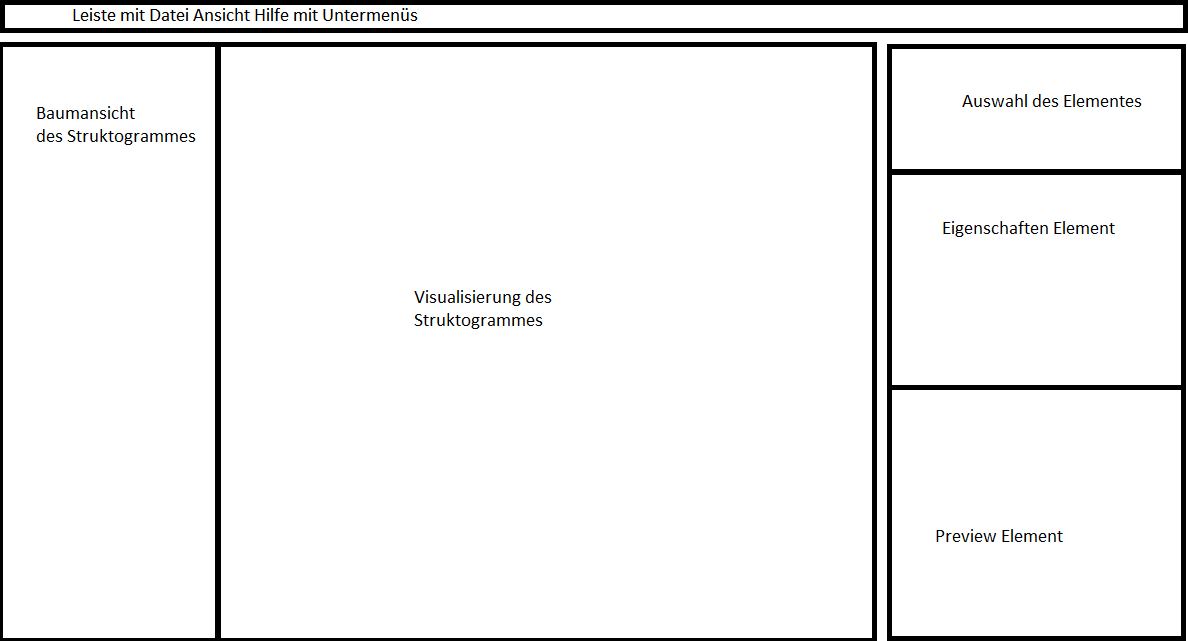
\includegraphics[width=1.3\textwidth]{gui-skizze.png}
\end{figure}
\begin{itemize}

\item (1) Baumstruktur: Anzeigen von allen Elementen innerhalb des Struktogrammes in hieraischer Form.
\item (2) Standard Windowsdialogleiste
\item (3) Anzeigen des gesamten Struktogrammes
\item (4) Auswahl, welches Element hinzugefügt werden soll
\item (5) Auswahl, der Eigenschaften, des Elements
\item (6) Anzeigen einer Vorschau des Aktuellen Elements

\end{itemize}
\section{Qualitätszielbestimmung}

\begin{center}
  \begin{tabular}{| l | l | l | l | l |}
    \hline
   	 Produktqualität & Sehr Gut & Gut  & Normal & Nicht Relevant \\ \hline
    	 Funktionalität &   &  x &  & \\ \hline
 	 Zuverlässigkeit & x  &   &  & \\ \hline
 	Benutzbarkeit &   &  x &  & \\ \hline
      	 Effizienz &   &  x &  & \\ \hline
      	 Änderbarkeit &   &  &  x & \\ \hline
      	Übertragbarkeit &   &   &  & x \\ \hline
  \end{tabular}
\end{center}

\section{Globale Testszenarien/Testfälle}
\begin{itemize}
\item  Erstellen eines Struktograms
\item  Laden/Speichern eines Struktograms
\item  Exportieren eines Struktograms (Wunschkriterium)
\end{itemize}
\section{Entwicklungsumgebung}
\subsection{Software}
\begin{itemize}
\item Visual Studio 2015
\item git in Kombination mit github.com
\item UML-Designer
\end{itemize}
\section{Verteilung der Aufgaben zwischen den Projektteilnehmer}
F10-F40 Martin Plank
F50-F80 Christian Sacher
F90-F120 Jonas Toth


\section{Glossar}
Elemente des Struktogrammes und ihrer Darstellung
\begin{itemize}
% u read here https://de.wikipedia.org/wiki/Nassi-Shneiderman-Diagramm
	\item Sequenz\\
	
	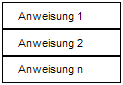
\includegraphics[scale=1]{LineareAnw.png} 
	\item Einfache Verzweigung\\
	
	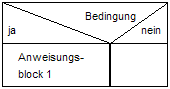
\includegraphics[scale=1]{EinfAusw.png} 
	\item Alternative Verzweigung\\
	
	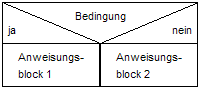
\includegraphics[scale=1]{ZweifAusw.png}
	\item Fallauswahl\\
	
	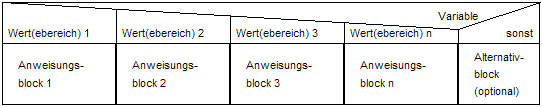
\includegraphics[scale=1]{Fallauswahl.png} 
	\item Zählergesteuerte Schleife\\
	
	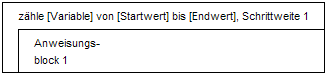
\includegraphics[scale=1]{Zaehlschleife.png} 
	\item Kopfgesteuerte Schleife\\
	
	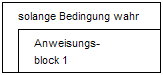
\includegraphics[scale=1]{KopfgesteuerteSchleife.png} 
	\item Fußgesteuerte Schleife\\
	
	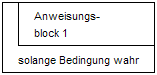
\includegraphics[scale=1]{FussgesteuerteSchleife.png} 
	\item Endlosschleife\\
	
	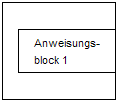
\includegraphics[scale=1]{Endlosschleife.png} 
	\item Aussprung\\
	
	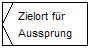
\includegraphics[scale=1]{Aussprung.png} 
	\item Aufruf\\
	
	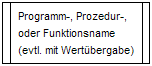
\includegraphics[scale=1]{Aufruf.png} 
	
	Quelle: https://de.wikipedia.org/wiki/Nassi-Shneiderman-Diagramm 01.12.2015
\end{itemize}
\end{document}
